\section{Introduction}
Strong gravitational lensing by a galaxy splits a gravitational-wave (GW) signal into two or more images with the same waveform, arriving minutes to months apart, with different amplitudes and with phase shifts of $0$, $\pi/2$ or $\pi$ set by the image type \citep{takahashi2003waveeffects,dai2017morse,ezquiaga2021phase}. About one in a thousand binary-black-hole (BBH) signals at current sensitivity is expected to be lensed in this way \citep{ng2018rates,oguri2018distribution,wierda2021beyond}. Searches of the LIGO--Virgo--KAGRA (LVK) data through the fourth observing run have found no confident pair \citep{hannuksela2019search,lvk2021o3a,lvk2024o3search,lvk2025gwtc4lensing}. These searches ask whether two events are consistent with being images of one source. They do not use the information that galaxies able to produce the observed delay are, for a growing fraction of the sky, already known: the lens catalogues built from SDSS, DESI, HSC and Euclid imaging and spectroscopy list tens of thousands of confirmed and candidate galaxy-scale lenses with measured Einstein radii and redshifts \citep{bolton2008slacs,sonnenfeld2018sugohi,huang2021desi,euclid2025q1lenses}. A lensed GW pair whose host is one of these systems is the case in which the time delay and the relative magnification can be turned into a measurement of the Hubble constant \citep{liao2017precision,paper1,paper2}.

Here we search the public LVK data for such pairs. The search has two stages. The first ranks every pair of events by a statistic that compares the GW observables of the two events with the prediction of each catalogued lens, and estimates the chance level of the best coincidences by rotating the lens catalogue on the sky. The second analyses the best pairs with a joint Bayesian fit of both signals to the detector strain, and calibrates the resulting coherence ratio with unrelated simulated events in real noise that pass the same selection. We also measure, with lensed signals from a realistic population injected into the same noise, the fraction of lensed pairs the search would recover.

\section{Data}
\label{sec:data}
\emph{GW events.} We use every public event with released parameter-estimation (PE) samples: GWTC-2.1 and GWTC-3 for O1--O3, GWTC-4.1 for O4a and GWTC-5.0 for O4b \citep{lvk2024gwtc21,lvk2023gwtc3,lvk2025gwtc4,lvk2026gwtc5}, 283 events in total, together with the O4c event GW250207 \citep{lvk2026gw250207}. For each event we take the samples of the LVK fiducial analysis (\textsc{IMRPhenomXPHM}, with its precession model), the power spectral densities (PSDs), the sky map and the analysis settings. Because a lensed partner may be too faint to enter the catalogues, we add the 492 sub-threshold candidates of the O4a and O4b searches with astrophysical probability above 0.1, for which only the search sky map and template masses exist, and the 67 significant public alerts of O4c, for which only sky maps are public. In total 842 events and candidates enter stage~1.

\emph{Strain.} The second stage uses the public strain of GWOSC \citep{gwosc2023} around each event, with the detectors, segment length, sampling rate and frequency band of the LVK analysis of that event. The LVK analyses of several events used strain from which a glitch had been subtracted; these cleaned data are not public, with consequences described in Sec.~\ref{sec:dq}.

\emph{Lens catalogue.} We merge the public strong-lens catalogues and candidate lists---the spectroscopic lens samples (SLACS, BELLS, SL2S and 24 further samples served by VizieR \citep{bolton2008slacs,brownstein2012bells}), the DESI spectroscopic searches \citep{hsu2026desipairs,karp2026desisfl}, the HSC searches SuGOHI and HOLISMOKES \citep{sonnenfeld2018sugohi,schuldt2025holismokes16}, Euclid Q1 \citep{euclid2025q1lenses}, the machine-learning candidate lists of the DESI Legacy Surveys, UNIONS, KiDS, DELVE and DES \citep{huang2021desi,stein2022mining,storfer2024desi,inchausti2025desi,storfer2025glue,grespan2024teglie,zaborowski2023delve,gonzalez2025des} and the lenscat compilation \citep{vujeva2024lenscat}---into one table of 48,739 systems, of which 10,342 are confirmed or high-grade candidates and 1,512 are clusters; entries within 5~arcsec are one system. Of the galaxy lenses, 6,964 have a lens redshift, a source redshift and an Einstein radius. For stage~1 each galaxy lens is described by its position, its Einstein radius $\theta_E$ (from the lensed arc, or from the velocity dispersion through the isothermal relation) and its lens redshift $z_l$; the source redshift of the arc is used only as a prior on the GW source redshift, since the GW host need not be the arc.

\section{Stage 1: ranking all pairs against the known lenses}
\label{sec:stage1}
For a pair of events $a$ (earlier) and $b$ (later) we compute three quantities. The first, $\ln B_{\rm ms}$, is the overlap of the posteriors of the detector-frame chirp mass, mass ratio and effective spin, divided by the prior \citep{haris2018identifying}; it measures whether the two signals could come from the same binary. The second, $\ln B_{\rm sky}$, is the overlap of the two sky maps on an isotropic prior. The third is the lens term. A catalogued lens $L$ with Einstein radius $\theta_E$ and redshift $z_l$, modelled as a singular isothermal sphere, produces two images of a source at scaled position $y<1$ with magnifications $1\pm1/y$ and delay $\Delta t=2y\theta_E^2D_{\Delta t}(z_l,z_s)/c$, where $D_{\Delta t}$ is the time-delay distance. The observed delay therefore fixes $y$ and the two magnifications, and the source redshift fixes the luminosity distance, so the lens predicts the apparent distances $d_L/\sqrt{|\mu|}$ that each event measures. The lens term $\Lambda_L$ is the probability density of the observed delay and of the two measured apparent distances under this prediction, marginalised over the unknown source redshift with the lensed-source redshift distribution, divided by the same density under the unrelated-event hypothesis (uniform delay within the observing time, independent distances). Summing over the lenses inside the common sky region of the pair, weighted by $\theta_E^2$ (the lensing cross-section),
\begin{equation}
\ln B_{\rm cat}=\ln B_{\rm ms}+\ln\Big[\sum_L\pi_L\,(4\pi)^2\,p_a(\boldsymbol\Omega_L)\,p_b(\boldsymbol\Omega_L)\,\Lambda_L\Big]
\label{eq:bcat}
\end{equation}
is the ranking statistic for ``lensed by a catalogued lens''. A companion statistic $\ln B_{\rm pop}$ replaces the catalogue by the full galaxy population (the $\sigma_v^4$-weighted velocity-dispersion function, \citep{choi2007vdf}) and the sky overlap $\ln B_{\rm sky}$, and ranks pairs for ``lensed by any galaxy''. For sub-threshold candidates without PE the mass term uses the template chirp mass with a 15\% width and the sky term the search sky map.

The chance level of $\ln B_{\rm cat}$ is measured by rotating the whole lens catalogue in right ascension 200 times and recomputing the statistic of every pair; the fraction of rotations whose largest value exceeds the observed largest value is the probability that a coincidence this strong arises by chance. For $\ln B_{\rm pop}$ the background comes from 50 reassignments of the event times.

\emph{Validation.} For the 3,570 O4a pairs analysed by the LVK lensing search \citep{lvk2025gwtc4lensing}, our $\ln B_{\rm ms}+\ln B_{\rm sky}$ and the LVK posterior-overlap statistic have a Spearman rank correlation of 0.94. The three O4a pairs the LVK search followed up rank 5th, 14th and 21st of the 9,978 PE--PE pairs in $\ln B_{\rm pop}$.

\emph{Result.} Of the 354,061 pairs with delays below one year, 66,232 pass the loose consistency cuts ($\ln B_{\rm ms}>0$, $\ln B_{\rm sky}>-2$). The largest $\ln B_{\rm cat}$ is 11.4 (GW241204\_154600 and the sub-threshold candidate GW241204\_182859, 2.7~h apart), exceeded in 57\% of catalogue rotations; the largest among PE--PE pairs is 11.4 (GW231113\_200417 and GW231223\_202619), also $p=0.57$. The largest $\ln B_{\rm pop}$ is 9.9 (two sub-threshold O4b candidates 50~min apart, $p=0.73$). No pair is a significant coincidence with a known lens or with the galaxy population (Fig.~\ref{fig:stage1}).

\begin{figure}
\centering
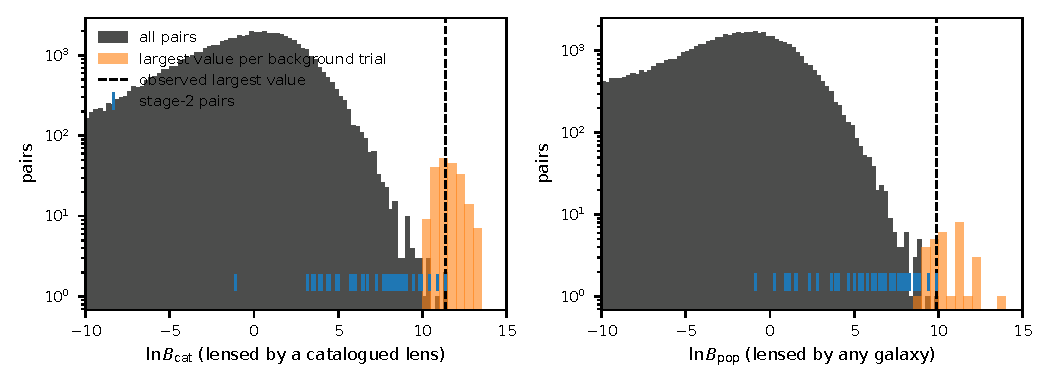
\includegraphics[width=\columnwidth]{figures/fig_stage1.pdf}
\caption{Stage~1. Left: distribution of $\ln B_{\rm cat}$ over all pairs (dark) and of the largest value in each rotation of the lens catalogue (orange); dashed: the observed largest value. Right: the same for $\ln B_{\rm pop}$, with the background from reassigned event times. Ticks: the pairs analysed in stage~2.}
\label{fig:stage1}
\end{figure}

\section{Stage 2: joint analysis of the strain}
\label{sec:stage2}
The 25 best pairs by $\ln B_{\rm cat}$ and the 25 best by $\ln B_{\rm pop}$ among events with LVK PE (43 distinct pairs, 67 events), and 13 pairs of sub-threshold candidates with delays below two days, are analysed on the strain. For each pair we run three Bayesian analyses with the same waveform (\textsc{IMRPhenomXPHM} with the precession model and frequency settings of the LVK analysis), the LVK PSDs, and the same prior ranges: image $A$ alone, image $B$ alone, and both images jointly. In the joint model the two signals share all source parameters; image $B$ differs by its arrival time, by its amplitude ratio $\sqrt{\mu_B/\mu_A}$, and by its own image type (Morse phase). Each single-image model also carries a free image type, so that the three analyses differ only in whether the parameters are shared. The coherence ratio
\begin{equation}
\lnC=\ln Z_{\rm joint}-\ln Z_A-\ln Z_B
\label{eq:lnc}
\end{equation}
compares the lensed hypothesis with two unrelated events \citep{haris2018identifying,janquart2023golum}. The evidences come from nested sampling with 1000 live points; their statistical errors add to $\pm0.3$ in $\lnC$. For the sub-threshold candidates, which have no LVK PE, the PSD is estimated from 512~s of data around the candidate and the prior ranges from the search template. Our single-event likelihood reproduces the LVK maximum log-likelihood of each event to within 1--2 (calibration marginalisation excluded). Nested sampling of a two-detector event does not always cover the whole sky ring: our single-event posteriors contain a median 88\% (mean 82\%) of the LVK sky posterior mass, so individual evidences can be low by a few tenths. The background pairs (Sec.~\ref{sec:twins}) are sampled with 500 live points and carry the same error; repeating two background analyses with 1000 live points changes their $\lnC$ by $-0.18$ and $-0.02$. One real pair, GW231223\_075055 and GW241114\_235258, had not converged after 250~h of joint sampling and is not included; 55 pairs (42 PE pairs and 13 sub-threshold pairs) have $\lnC$.

\subsection{Background: unrelated pairs that pass the same selection}
\label{sec:twins}
A positive $\lnC$ does not by itself indicate lensing: when two posteriors overlap, the joint model is rewarded for sharing fifteen parameters even if the events are unrelated. The pairs that reach stage~2 were chosen \emph{because} their posteriors overlap, so the null distribution of $\lnC$ must be measured on unrelated pairs that pass the same selection.

We build such pairs from simulated unlensed events in real noise. For each stage-2 pair we draw one sample from the LVK posterior of each event and inject it into O4 detector noise at a time with no catalogued event, rotating the right ascension so that the signal keeps its position relative to the detectors. Each of these 96 simulated events is analysed alone with the stage-2 settings; the 80 with a maximum log-likelihood above 28 (signal-to-noise ratio $\gtrsim7.5$, the level of all but one real stage-2 event) are realistic detections. We pair every two of them that come from different real events (3118 pairs), compute the stage-1 statistics with the time delay of the parent events, and keep the pairs above the stage-2 selection thresholds. These 16 pairs (0.5\% of all pairs, against 1.0\% for the real events) receive the joint analysis; the single-image evidences are reused, rescaled to the prior of the new pairing, which differs only in the chirp-mass and distance ranges.

Pairing the two simulated events of the \emph{same} stage-2 pair, without the selection, does not give a valid null. Each simulated event lies one posterior sample plus one new noise realisation away from its parent, so the two are less consistent than the real pair (their standardised chirp-mass separation is twice that of the real pairs), and their $\lnC$ is lower by a median of 4.7. Such pair-matched backgrounds make every real pair look significant.

\subsection{Efficiency: lensed pairs in real noise}
\label{sec:inject}
To measure what the search recovers, we simulate lensed BBHs from the GWTC-4.0 population and galaxy lenses from the velocity-dispersion function with elliptical power-law mass profiles and external shear, as in Paper~I \citep{paper1}. Of the lensed systems, only those whose two brightest images both reach a network signal-to-noise ratio (SNR) of 10 with the O4 sensitivity are kept: these are $2.2\times10^{-4}$ of all lensed systems, dominated by high magnifications ($|\mu|\approx20$ for both images, median), short delays (median 1~h, 95\% below 10~d) and quadruple-image configurations (72\%). The 135 pairs are injected, each image shifted by a whole number of sidereal days so that its detector response is unchanged, into real O4a and O4b noise, and analysed with the single-image settings of stage~2; their posteriors enter the stage-1 ranking exactly as the real events, and 45 pairs also receive the joint analysis.

\section{Data quality of the public strain}
\label{sec:dq}
The pair GW240601\_061200 and GW240612\_081540, 11 days apart, gave $\lnC=45.9\pm0.4$, far above every other pair. The joint fit converged to a template at 370~Mpc, nearly edge-on, with a magnification ratio of $e^{-3.8}$ and a maximum log-likelihood of 163, against 53 and 31 for the two single-image fits. Evaluating the single-image likelihood of GW240601\_061200 at the joint best fit gives 135: in the public Livingston strain this template has a matched-filter SNR of 16 where its optimal SNR is 13, i.e. it fits power that is not the GW signal. The LVK analysis of this event used Livingston data from which a glitch overlapping the signal had been subtracted with BayesWave; the public strain contains the glitch. The joint analysis, with its longer sampling run, found the glitch-fitting mode; the single-image run never did, and the difference appeared as coherence.

This failure can be detected without the cleaned data. For each event we compare the largest log-likelihood reached by our single-image analysis with the largest log-likelihood of the LVK posterior samples (Fig.~\ref{fig:dq}). For most events the two agree to within a few units, the expected gap between the maximum of 10,000 samples and the true maximum. An excess above 10 (20 for O3 events, whose released log-likelihoods are marginalised over time and distance) indicates power in the public strain that the LVK analysis did not see. For the 20 sub-threshold candidates, which have no LVK PE, the reference is $\rho^2/2$, with $\rho$ the network SNR of the search template; the best-fitting waveform exceeds it by a few units, and the same threshold of 10 applies. Eleven of the 90 events are flagged. Seven fail the comparison with the LVK samples: GW200322\_091133 ($+59$), GW240716\_034900 ($+58$), GW240615\_113620 ($+26$), GW240530\_012417 ($+22$), GW240601\_061200 ($+17$, and $+3216$ in the single-image run of another of its pairings), GW230805\_034249 ($+11$) and GW240512\_024139 ($+10$). Four sub-threshold candidates fail the comparison with the search: GW240615\_055016 ($+157$), GW240531\_111628 ($+85$), GW240925\_010025 ($+82$) and GW240406\_062847 ($+15$). A second test compares the maximum log-likelihood of the joint fit with the sum of the two single-image maxima; a positive excess means that a single-image run missed a mode. Three pairs fail it: the GW240601 pair ($+79$), GW240601\_061200 with GW240908\_125134 ($+29$) and GW230805\_034249 with GW230811\_032116 ($+8$), all with a flagged event. Pairs with a flagged event are excluded from the headline result and listed separately: 13 of the 55 pairs, leaving 42 clean pairs (34 PE pairs and 8 sub-threshold pairs).

The search test caught the second-highest value of the whole search. The sub-threshold pair GW240615\_023849 and GW240615\_055016, 3.2~h apart, gave $\lnC=25.7\pm0.5$. The search recorded GW240615\_055016 at $\rho=7.9$ ($p_{\rm astro}=0.17$) with a template chirp mass of 12.9; our analysis of its data reaches a maximum log-likelihood of 188 (an SNR near 19) at a detector-frame chirp mass of 6.55 and a distance of 82~Mpc, at the lower edge of its distance prior. In the joint fit the earlier image adds a log-likelihood of only 7 (38 in its own fit), whereas the data of GW240615\_055016 reach 217: the joint model places that image at 34~Mpc through the relative magnification, outside the prior of the single-image run. Restricting the earlier candidate to a chirp mass of 6.4--6.7 gives it $\ln B=0.0$, so the coherence is not shared signal; and repeating the single-image analysis of GW240615\_055016 with the distance prior extended to 10~Mpc drives the fit to that edge and to the lower edge of the mass ratio. Loud power that the template follows to the edges of the prior, at an SNR far above that of the search, is the signature of a non-Gaussian transient in the data, not of a GW signal.

\begin{figure}
\centering
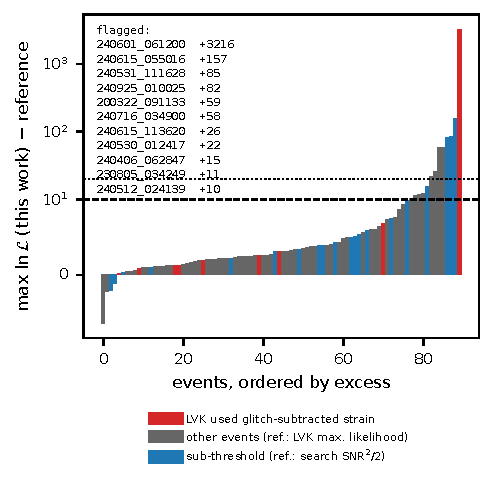
\includegraphics[width=\columnwidth]{figures/fig_dq.pdf}
\caption{Excess of the maximum log-likelihood of our single-image analysis over a reference, for the 90 events of stage~2: the LVK maximum-likelihood sample for events with LVK PE, and $\rho^2/2$ of the search template for sub-threshold candidates. Red: events whose LVK analysis used glitch-subtracted strain. Dashed (dotted): the threshold of the data-quality cut for O4 (O3) events.}
\label{fig:dq}
\end{figure}

\section{Results}
\label{sec:results}
Figure~\ref{fig:lnc} shows $\lnC$ for the 42 pairs with clean data against the background of unrelated selected pairs. The background is broad and positive: its median is 7.2, its 90th percentile 10.3 and its largest value 11.8. The real pairs follow it, with the same median of 7.2. Two pairs exceed every background value: GW250109\_010541 with GW250116\_015318 (7.0~d apart, $\lnC=13.4\pm0.3$) and GW250116\_015318 with GW250119\_025138 (3.0~d, $13.3\pm0.4$). Both contain GW250116\_015318, the faintest of the PE events in stage~2. Each has a per-pair $p=1/17$, the smallest value 16 background pairs can give, and, for 42 trials, a global false-alarm probability of 0.92. The published O4a candidates GW230707\_124047 with GW230708\_230935 and GW230922\_040658 with GW231005\_021030 give 8.1 and 7.1, at the median of the background. The 12 pairs in common with the LVK joint-PE follow-up \citep{lvk2025gwtc4lensing} have coherence ratios that rank similarly (Spearman 0.62), with a median offset of 9.2 (interquartile range 8.6--10.1) from the different priors on the relative magnification and delay. The stage-1 favourite among the sub-threshold pairs, GW240925\_000956 and GW240925\_010025 (50~min apart), gives $\lnC=-2.9$, and its later candidate fails the data-quality test.

\begin{figure}
\centering
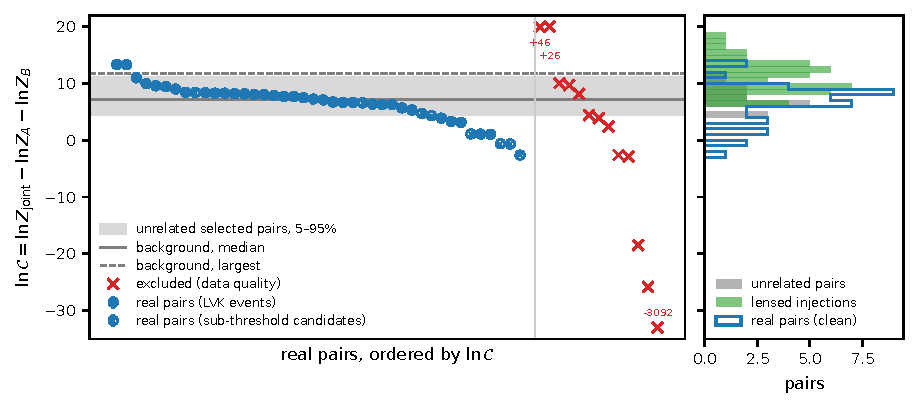
\includegraphics[width=\columnwidth]{figures/fig_lnc.pdf}
\caption{Coherence ratio of the real pairs (points, ordered by $\lnC$; open symbols: sub-threshold pairs; crosses: pairs excluded by the data-quality tests, with the values of those beyond the axes) against the background of unrelated selected pairs (gray band: 5--95\% range; solid line: median; dashed: largest value). Right: distributions for the background, the lensed injections and the clean real pairs.}
\label{fig:lnc}
\end{figure}

\emph{Efficiency and limit.} Of the 135 injected lensed pairs, 91\% pass the stage-1 cuts and 80\% rank above the stage-2 selection threshold in $\ln B_{\rm pop}$. If their lens were in the catalogue, 69\% would rank above the threshold in $\ln B_{\rm cat}$; 82\% are selected by one of the two statistics. Of the 45 injected pairs with joint analyses, 37 of them selected, the median $\lnC$ is 11.1. Of the selected ones, 43\% exceed the largest background value and 27\% exceed the largest clean real value, 13.4. Taking that loudest value as the detection threshold, the efficiency of the search for this population is $\epsilon=0.82\times0.27=0.22\pm0.06$. With no candidate above it, the number of lensed pairs in O4a and O4b with both images above SNR 10 is below $2.3/\epsilon\approx10$ at 90\% confidence. This bound is an order of magnitude above the expected number, which is of order one or less \citep{ng2018rates,wierda2021beyond}. The efficiency is limited by the width of the null distribution, not by the stage-1 selection: injected pairs whose fainter image has SNR below 12 have a median $\lnC$ of 9.8 and exceed the largest background value in 22\% of cases, against 52\% above SNR 12.

\begin{table*}
\centering
\caption{The ten clean pairs with the highest $\lnC$: events, delay, stage-1 statistics, coherence ratio, per-pair $p$-value against the 16 background pairs, and false-alarm probability after the 42 trials.}
\label{tab:top}
\begin{tabular}{llrrrrrr}
\toprule
Event $A$ & Event $B$ & $\Delta t$ [d] & $\ln B_{\rm cat}$ & $\ln B_{\rm pop}$ & $\ln\mathcal C$ & $p$ & FAP \\
\midrule
GW250109\_010541 & GW250116\_015318 & 7.0 & 4.9 & 6.8 & $13.4\pm0.3$ & 0.06 & 0.92 \\
GW250116\_015318 & GW250119\_025138 & 3.0 & 7.8 & 7.8 & $13.3\pm0.4$ & 0.06 & 0.92 \\
GW190805\_211137 & GW190916\_200658 & 42.0 & 10.0 & 8.8 & $11.0\pm0.3$ & 0.12 & 0.99 \\
GW230630\_125806 & GW230707\_124047 & 7.0 & 8.6 & 8.3 & $10.0\pm0.3$ & 0.18 & 1.00 \\
GW231231\_154016 & GW240531\_040326 & 151.5 & 8.0 & 1.5 & $9.6\pm0.3$ & 0.24 & 1.00 \\
GW230630\_125806 & GW240527\_183429 & 332.2 & 9.5 & 6.2 & $9.5\pm0.3$ & 0.24 & 1.00 \\
GW230630\_125806 & GW230709\_122727 & 9.0 & 7.3 & 7.2 & $9.0\pm0.3$ & 0.29 & 1.00 \\
GW231113\_200417 & GW231223\_202619 & 40.0 & 11.4 & 5.3 & $8.4\pm0.3$ & 0.35 & 1.00 \\
GW230825\_041334 & GW230826\_031533 & 1.0 & 3.9 & 8.0 & $8.4\pm0.3$ & 0.35 & 1.00 \\
GW231206\_233901 & GW240525\_031210 & 170.1 & 8.4 & 1.2 & $8.4\pm0.3$ & 0.35 & 1.00 \\
\bottomrule
\end{tabular}

\end{table*}

\section{Discussion}
\label{sec:discussion}
\emph{Catalogue conditioning.} Conditioning on the known lenses adds the predicted delay and apparent distances to the usual parameter overlap, and it ranks a pair whose lens is catalogued above most unrelated pairs: 69\% of the injected pairs would pass the stage-1 selection on $\ln B_{\rm cat}$ alone. Its reach is set by the completeness of the lens catalogues. These hold tens of thousands of systems, a small fraction of the galaxies able to lens a GW source, and Euclid and LSST will enlarge them by an order of magnitude.

\emph{The null distribution of $\lnC$.} Unrelated pairs selected for overlapping posteriors have a coherence ratio near $+7$, and their largest values exceed 11. A fixed threshold on $\lnC$ therefore has no meaning, and neither does a background built pair by pair without the selection: it sits about 5 units lower and makes every real pair look significant. The selection-matched background costs one single-image analysis per simulated event and one joint analysis per selected pair. With 16 pairs it limits the per-pair $p$-value to about 0.06, so a confident detection would need a background larger by a factor of $\sim10^2$.

\emph{The public strain.} Glitch mitigation is part of the LVK analyses but not of the strain release. In our search, glitches produced the two largest coherence ratios, 45.9 and 25.7, both larger than the largest value among the 45 lensed injections, 18.2. Searches on public data must either obtain the mitigated frames or apply a likelihood-excess test like the one used here, against the LVK maximum likelihood for catalogued events and against the search SNR for sub-threshold candidates.

\emph{What a detection would give.} For a pair with an identified lens, the measured delay and magnification ratio together with the lens model give the Hubble constant from a single system \citep{paper2}. The O4c strain, to be released at the end of 2026, and O5 will add events at the same and higher sensitivity, to be ranked against lens catalogues that Euclid and LSST will enlarge.

\section{Conclusions}
We have searched all public LVK data, 842 events and candidates from O1 to O4, for strongly lensed pairs, ranking every pair against 47,227 catalogued galaxy lenses and analysing the 56 best pairs jointly on the public strain. No pair is significant: the largest stage-1 coincidence is reproduced by chance in 57\% of catalogue rotations, and the largest clean coherence ratio, $\lnC=13.4$, has a false-alarm probability of 0.92 against unrelated simulated pairs that pass the same selection. That background has a median $\lnC$ of 7.2; backgrounds built without the selection are about 5 units lower and would have made every real pair look significant. In public strain, unmitigated glitches give the largest spurious coherence ratios, and a comparison of the maximum likelihood with the LVK analysis or with the search SNR identifies them.
